% Dharma: IEEE conference paper (IEEEtran, at most 8 pages).
% Build: make -C docs paper  (output: docs/build/paper/dharma.pdf)
\documentclass[conference]{IEEEtran}

\usepackage{cite}
\usepackage{amsmath,amssymb}
\usepackage{graphicx}
\usepackage{booktabs}
\usepackage{xcolor}
\usepackage{url}
\usepackage[hidelinks]{hyperref}

% Author and affiliations of every Dharma document (paper and manual). Change them here only.
\newcommand{\DharmaAuthor}{I Wayan Agus Darmawan}
\newcommand{\DharmaEmail}{darmawandeveloper@gmail.com}
\newcommand{\DharmaAffilOne}{Department of Computer Engineering, Institut Teknologi Sepuluh
  Nopember (ITS), Surabaya, Indonesia}
\newcommand{\DharmaAffilTwo}{PT Ezra Robotics Teknologi, Indonesia}
\newcommand{\DharmaVersion}{0.2.0}

% Macros shared by the paper and the manual (needs xcolor and amsmath).

% Placeholder for content that phase 2 fills in (measured results, test names). Renders in red
% so nothing unfinished goes unnoticed.
\newcommand{\todo}[1]{\textcolor{red}{\textbf{[TODO:} #1\textbf{]}}}
% A number still to be measured, for tables.
\newcommand{\tbd}{\textcolor{red}{\textbf{??}}}

% Names
\newcommand{\pkg}[1]{\texttt{#1}}
\newcommand{\topic}[1]{\texttt{#1}}
\newcommand{\frm}[1]{\texttt{#1}}
\newcommand{\param}[1]{\texttt{#1}}

% Math
% {}^{a}T_{b}: pose of frame b in frame a (maps points from b to a), the TF edge a -> b.
\newcommand{\T}[2]{{}^{#1}\mathbf{T}_{#2}}
\newcommand{\R}{\mathbb{R}}
\newcommand{\SE}[1]{\mathrm{SE}(#1)}
\newcommand{\vect}[1]{\boldsymbol{#1}}
\newcommand{\tr}{t_{\mathrm{r}}}
\newcommand{\amax}{a_{\mathrm{dec}}}


\graphicspath{{../diagrams/pdf/}}

\begin{document}

\title{Dharma: A Robot-Agnostic, Safety-Layered ROS~2 Autonomy Stack for Service Robots in
  Crowded Public Spaces}

\author{\IEEEauthorblockN{\DharmaAuthor$^{1,2}$}
\IEEEauthorblockA{$^{1}$\DharmaAffilOne\\
$^{2}$\DharmaAffilTwo\\
\DharmaEmail}}

\maketitle

\begin{abstract}
Service robots that guide, inspect or deliver in malls, stations and offices drive among people
on legs or wheels, and the software that moves them is usually written for one robot. We
present Dharma, an open ROS~2 autonomy stack (Foxy, Humble and Jazzy) that separates what is generic
from what is robot-specific: one robot profile (footprint, base height, kinematics, limits,
frames) is the single source of every geometric and dynamic assumption, typed and validated
configuration replaces untyped parameters, and algorithm families are plugins. The stack
combines LiDAR-inertial odometry behind a gravity-aligned bridge, a fiducial-anchored SE(2)
extended Kalman filter over the map-to-odometry correction with chi-square gating, log-odds
mapping with jump and correction gating, footprint-aware A* planning, path tracking with a
Frenet path shift around people, and a protective field that limits translation, rotation and
their combination with a single braking model shared by every speed limit in the stack. Sensing
is fail-safe by construction: a blind or stale sensor is an obstacle, never free space. We
describe the models, the software engineering that keeps them consistent (pure cores,
module-size and purity checks, a Foxy, Humble and Jazzy CI matrix), and a seeded simulation protocol
for stopping distance, blind-sensor behaviour, localization error and avoidance performance.
In seeded simulations the field kept its margin, a LiDAR without returns zeroed the command
within 0.13~s, the filter cut the localization error from 0.43 to 0.07~m, and path shift
passed people in 37 of 40 runs; the runs also exposed defects, which we report.
\end{abstract}

\begin{IEEEkeywords}
service robots, legged robots, ROS~2, localization, speed and separation monitoring, software
architecture
\end{IEEEkeywords}

\section{Introduction}
\label{sec:intro}

Robots that guide visitors, patrol or carry goods in public buildings share their space with
crowds that do not watch out for them~\cite{burgard1999museum,triebel2016spencer,
kruse2013humanaware}. Quadruped platforms are attractive there: they climb thresholds and
ramps and are perceived as approachable, but their bodies pitch and roll with the gait, their
footprint is long compared with its width, and their drivers expose only a velocity command.
Products built on such platforms tend to grow their autonomy around one robot: the footprint is
repeated in five parameter files, the base height is assumed in two different values, frames
are hard-coded, and safety checks that were right for one speed are silently wrong for the next.

Dharma grew out of such a product (a tour-guide robot) and was refactored into a general,
robot-agnostic stack. An independent review of the original code modelled every subsystem and
found three structural weaknesses: pose estimates carried no uncertainty and were never
corrected continuously against the map; geometric assumptions (robot radius, base height,
level frames) were inconsistent across packages; and the robot description was scattered, so
the stack was not robot-agnostic in practice. It also found safety defects: a planner radius
smaller than the robot's half diagonal, a protective field that ignored rotation, and blind
sensors read as free space. This paper describes the redesigned stack (v0.2.0) and the models
behind it.

\textbf{Contributions.}
\begin{itemize}
  \item A layered, robot-agnostic architecture in which one robot profile is the single source
    of geometry, limits and frames, with typed configuration validated at start and on every
    change, typed status interfaces and plugin registries (Sec.~\ref{sec:arch}).
  \item A gravity-aligned bridge for LiDAR-inertial odometry and a fiducial-anchored SE(2)
    extended Kalman filter over the map-to-odometry correction: drift grows with motion, not
    time, the innovation is taken where the robot is, and a chi-square gate opens with the
    uncertainty (Sec.~\ref{sec:loc}).
  \item One braking model shared by the speed profile, the path shift and a protective field
    that limits translation, rotation and combined motion, with fail-safe sensing semantics and
    a latched e-stop that must be re-armed (Secs.~\ref{sec:track}--\ref{sec:field}).
  \item The engineering that keeps the models consistent: pure algorithm cores, enforced module
    size and purity, a ROS~2 Humble and Jazzy CI matrix, and traceability of every review
    finding to a fix and a regression test (Sec.~\ref{sec:eng}).
  \item A seeded simulation protocol with odometry drift, latency and sensor dropout to evaluate
    stopping, blind-sensor behaviour, localization and avoidance (Sec.~\ref{sec:eval}).
\end{itemize}

\section{Related Work}
\label{sec:related}

\textbf{Navigation frameworks.} ROS~2~\cite{macenski2022ros2} and its navigation system
Nav2~\cite{macenski2020marathon2,macenski2023survey} provide behaviour-tree navigation,
costmap layers, planners and controllers such as regulated pure pursuit~\cite{macenski2023rpp}.
Dharma is smaller in scope and complementary: it targets a robot class (legged and
omnidirectional service robots driven through a velocity interface) and puts the emphasis on a
single robot description, uncertainty-aware localization and a separate safety layer whose
limits are derived from the same braking model as the planner and the follower. The transform
library tf~\cite{foote2013tf} carries every frame; we add per-edge age diagnosis on top.

\textbf{LiDAR-inertial odometry.} FAST-LIO2~\cite{xu2022fastlio2} is an iterated error-state
Kalman filter with direct point-to-plane updates; LIO-SAM~\cite{shan2020liosam} uses smoothing
and mapping; Leg-KILO~\cite{ou2024legkilo} adds leg kinematics for dynamic legged robots. These
estimators take their world frame from the first IMU samples, so a robot that starts tilted
produces a tilted world; Dharma levels it explicitly in a static bridge.

\textbf{Fiducial localization and scan matching.} AprilTag~\cite{olson2011apriltag,
wang2016apriltag2} gives the pose of a known marker; the EKF formulation and chi-square gating
follow~\cite{barshalom2001estimation,thrun2005probabilistic}. Correlative scan matching on a
likelihood field~\cite{olson2009csm} supplies continuous corrections against the map.
Occupancy grids~\cite{elfes1989occupancy} with log-odds updates are the map representation;
graph-based systems such as Cartographer~\cite{hess2016cartographer} and SLAM
Toolbox~\cite{macenski2021slamtoolbox} close loops, which Dharma leaves for future work.

\textbf{Planning, tracking and reactive avoidance.} A*~\cite{hart1968astar} on an inflated
costmap, pure pursuit~\cite{coulter1992purepursuit}, the Stanley
controller~\cite{thrun2006stanley} and MPPI~\cite{williams2017mppi} are the path-level
building blocks; vector field histograms~\cite{borenstein1991vfh}, potential
fields~\cite{khatib1986potential}, follow-the-gap~\cite{sezer2012ftg} and the dynamic window
approach~\cite{fox1997dwa} are classical reactive methods. Lateral offsets in a Frenet
frame~\cite{werling2010frenet} let a robot pass an obstacle while keeping its route.

\textbf{Safety.} Speed and separation monitoring limits speed so the robot can stop before a
person reaches it~\cite{isots15066,marvel2016ssm}. Certified functions follow ISO
13849-1~\cite{iso13849} or IEC 61508~\cite{iec61508}, and personal care robots
ISO 13482~\cite{iso13482}. Dharma's protective field is a software channel modelled on speed
and separation monitoring; it is explicitly the second channel next to a hardware e-stop and a
safety-rated scanner, not a certified function.

\section{Architecture}
\label{sec:arch}

\begin{figure*}[t]
  \centering
  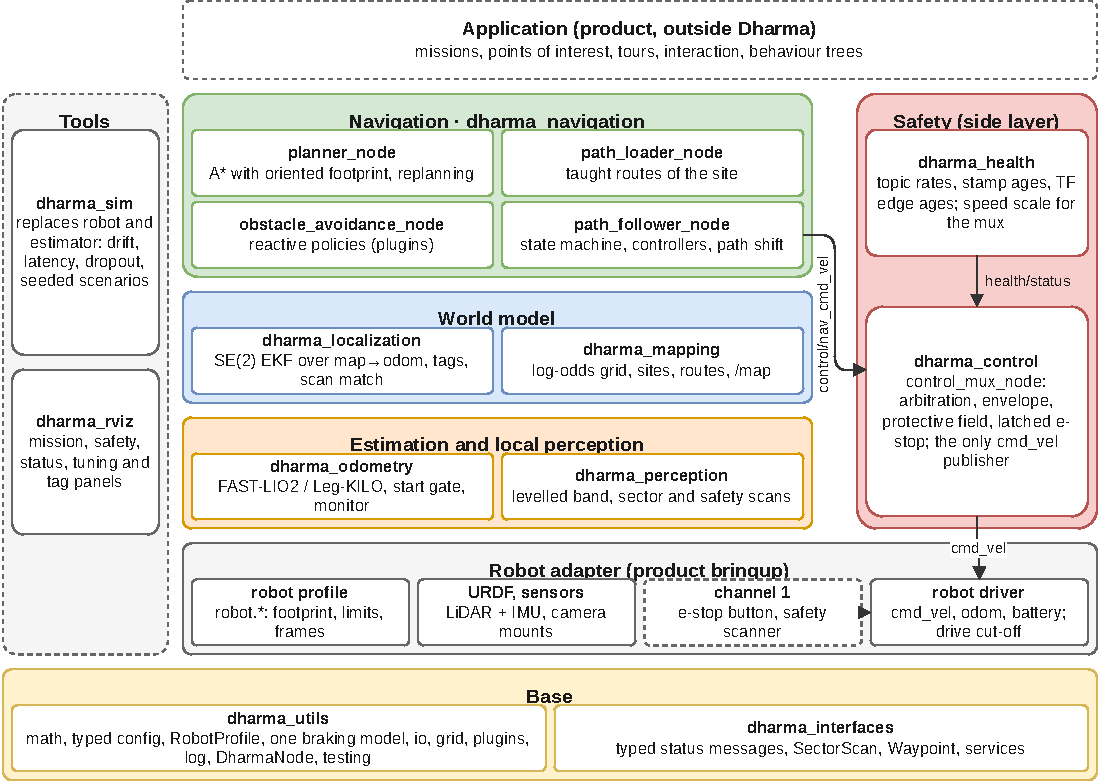
\includegraphics[width=0.92\textwidth]{layers}
  \caption{Layers of Dharma. Every layer depends only on the layers below it and on the base
    (\pkg{dharma\_utils}, \pkg{dharma\_interfaces}); the safety layer sits beside them and is
    the last gate before the robot driver. Colours: estimation orange, world model blue,
    navigation green, safety red, base yellow, hardware grey.}
  \label{fig:layers}
\end{figure*}

\textbf{Layers.} Fig.~\ref{fig:layers} shows the stack. The robot adapter belongs to the product
(driver, URDF, sensor mounts and the robot profile). Estimation and local perception turn raw
LiDAR, IMU and camera data into odometry and obstacle sectors around the robot; the world model
holds the map, the sites and the correction from odometry to the map; navigation plans and
follows paths and docks onto a fiducial-marked charger. Safety is a separate package beside all
layers: one control multiplexer is the only publisher of the robot's velocity command, and a
health monitor turns degraded sensing into a requested speed scale. Each repository depends only on the two base packages, and the
product bringup composes the package launch files.

\textbf{One robot profile.} Every node reads the same \param{robot.*} parameters, parsed into
an immutable \texttt{RobotProfile}: kinematics (omnidirectional or differential), base height
above the floor, a rectangular footprint (front, rear, half width), motion limits (speeds,
acceleration, braking deceleration, yaw deceleration, reaction time) and frame names. Derived
quantities are computed, not copied: the inscribed radius $r_{\mathrm{in}} = \min(f, b, w)$,
the circumscribed radius $r_{\mathrm{c}} = \sqrt{\max(f,b)^2 + w^2}$, the self filter of
perception and mapping, the height band above the floor, the lateral speed limit
($v_y = 0$ for differential robots). For the default profile ($f = b = 0.40$~m, $w = 0.28$~m)
$r_{\mathrm{in}} = 0.28$~m and $r_{\mathrm{c}} = 0.49$~m; the original planner used
$0.35$~m, so a path it accepted could swing a corner of the body about 14~cm into a wall while
turning. The profile validates cross-field consistency (no lateral speed for a differential
robot, distinct frames).

\textbf{Typed configuration.} Each node declares its parameters as frozen dataclasses whose
fields carry a default, unit, range, choices, description and a \emph{live} flag. The node
helper turns them into ROS parameter descriptors, validates every value at start and on every
\texttt{ros2 param set} (rejecting it with a reason), reports unknown parameters (typos) and
makes safety values read-only at runtime. A node that receives an invalid safety parameter
refuses to start instead of running with a default.

\textbf{Plugins and typed interfaces.} Controllers and avoidance policies implement abstract
base classes and register in a named registry that is also open to Python entry points, so a
product adds an implementation without forking. All status topics are typed messages with enum
constants (odometry, localization, mapping, site, planner, navigation, control, health) instead
of strings; safety-relevant actions are separate trigger services so that a default request
can never release or stop something.

\begin{figure}[t]
  \centering
  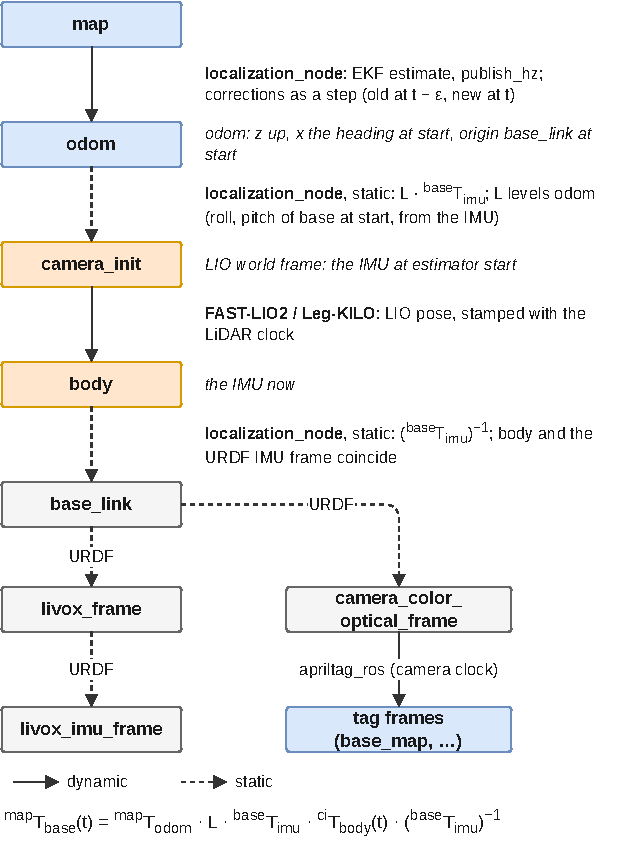
\includegraphics[width=\columnwidth]{tf_tree}
  \caption{TF tree. The LiDAR-inertial odometry publishes \frm{camera\_init}$\to$\frm{body};
    localization adds the static bridge (with the level rotation $L$) and the map correction.}
  \label{fig:tf}
\end{figure}

\textbf{Frames.} The tree follows REP-105 (Fig.~\ref{fig:tf}):
\frm{map}$\to$\frm{odom}$\to$\frm{camera\_init}$\to$\frm{body}$\to$\frm{base\_link}, where
\frm{camera\_init} is the IMU frame at estimator start and \frm{body} the IMU now. The pose of
the robot in the map is
\begin{equation}
  \T{map}{base}(t) = \T{map}{odom}\; L\, \T{base}{imu}\; \T{ci}{body}(t)\;
  \T{imu}{base},
  \label{eq:chain}
\end{equation}
with the static mounting $\T{base}{imu}$ from the URDF, $\T{imu}{base}$ its inverse and the
level rotation $L$ of Sec.~\ref{sec:bridge}. Frame names come from the profile; nothing is hard-coded.

\section{Methods}
\label{sec:methods}

\subsection{Gravity-aligned odometry bridge}
\label{sec:bridge}

FAST-LIO2~\cite{xu2022fastlio2} (or Leg-KILO~\cite{ou2024legkilo}) estimates
$\T{ci}{body}(t) \in \SE{3}$ with the world frame \frm{camera\_init} equal to the IMU frame at
start. If the robot starts tilted by $\theta$, that world is tilted: a horizontal distance $s$
appears as a height change and a shorter planar distance,
\begin{equation}
  \Delta z \approx s \sin\theta, \qquad \frac{\Delta s_{xy}}{s} = 1 - \cos\theta ,
  \label{eq:tilt}
\end{equation}
i.e.\ 3.5, 8.7 and 13.9~cm of false height per metre for $\theta = 2^\circ, 5^\circ,
8^\circ$. Mapping and perception filter obstacles in a height band above the floor and
assume a level frame, so a start at the previous 8° limit puts the floor 5~m ahead 0.7~m above
the band. Two measures remove this. A launch prefix holds the estimator (and every respawn)
until the IMU is still and level: largest angular rate below 0.03~rad/s, relative standard
deviation of $\|\vect{f}\|$ below 1\,\%, tilt at most 3°. Then localization measures the mean
specific force $\bar{\vect{f}}$ over a still window and computes the up direction of the base at
start, $\vect{u} = \mathbf{R}^{\mathrm{base}}_{\mathrm{imu}}\, \mathbf{R}^{\mathrm{ci}}_{
\mathrm{body}}(t)\, \bar{\vect{f}} / \|\cdot\|$. The level rotation $L$ is the rotation that
aligns $\vect{u}$ with $\vect{z}$, with its yaw removed so that \frm{odom}'s $x$ axis keeps the
start heading. The bridge publishes
\begin{equation}
  \T{odom}{ci} = L\, \T{base}{imu}, \qquad \T{body}{base} = \big(\T{base}{imu}\big)^{-1},
\end{equation}
so $\T{odom}{base}(t_0) = L$: \frm{odom} starts at \frm{base\_link}, with $z$ against gravity.
After an estimator restart it is levelled again. Only the direction of $\bar{\vect{f}}$ is used,
so accelerometer units do not matter.

The odometry monitor compares the estimator speed with the robot's own odometry as a residual
test~\cite{page1954cusum}:
\begin{equation}
  \begin{aligned}
    r_k &= v^{\mathrm{lio}}_k - v^{\mathrm{leg}}_k, \qquad
    \chi^2_k = \frac{r_k^2}{\sigma_{\mathrm{lio}}^2 + \sigma_{\mathrm{leg}}^2},\\
    S_k &= \max\big(0,\ S_{k-1} + \chi^2_k - \kappa\big),
  \end{aligned}
  \label{eq:cusum}
\end{equation}
with an alarm while $S_k > h$ ($\kappa = 3.84$, the 95\,\% quantile of $\chi^2_1$, $h = 20$).
The thresholds follow from the sensor variances, not from robot speeds. A restart is detected
only when the pose returns to the origin after a message gap or a physically impossible
translation jump; a yaw change alone (turning in place near the start) never counts.

\subsection{Fiducial-anchored SE(2) EKF}
\label{sec:loc}

\begin{figure}[t]
  \centering
  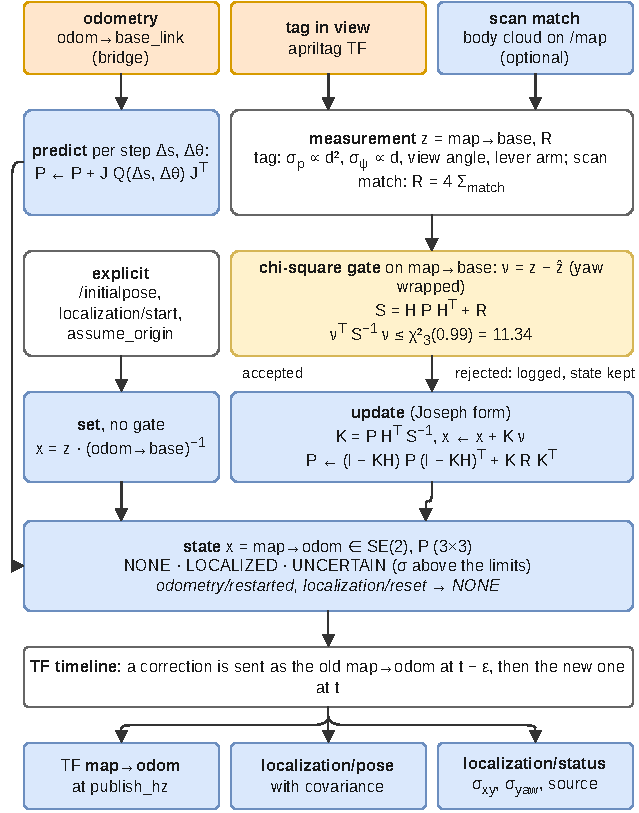
\includegraphics[width=\columnwidth]{localization_ekf}
  \caption{Localization: an EKF over \frm{map}$\to$\frm{odom}, predicted by odometry motion and
    corrected by fiducials, scan matching and explicit operator input.}
  \label{fig:ekf}
\end{figure}

The original stack replaced \frm{map}$\to$\frm{odom} by every tag detection, without
uncertainty and with ad-hoc rejection thresholds (0.5~m, 15°) that compared the correction
itself. A heading error $\delta\psi$ of that correction displaces the robot by
$e_\perp \approx L\,\delta\psi$ after a distance $L$ from the tag (17.5~cm after 10~m at
$\delta\psi = 1^\circ$), and a small rotation of \frm{map}$\to$\frm{odom} far from the odometry
origin moves the robot metres. Dharma estimates the correction itself (Fig.~\ref{fig:ekf}).

\textbf{State and prediction.} The state is $\vect{x} = (x, y, \psi)$ of $\T{map}{odom}$ with a
$3\times3$ covariance $\mathbf{P}$. With the odometry pose $\vect{o} = \T{odom}{base}$, the
robot pose is $h(\vect{x}) = \vect{x} \oplus \vect{o}$ and its Jacobian with respect to the state
\begin{equation}
  \mathbf{H} = \begin{bmatrix} 1 & 0 & -(y_b - y) \\ 0 & 1 & x_b - x \\ 0 & 0 & 1 \end{bmatrix}
\end{equation}
contains the lever arm from the \frm{odom} origin to the robot $(x_b, y_b)$. Drift is
proportional to motion: the odometry is counted in steps of distance $\Delta s$ and rotation
$\Delta\theta$, and
\begin{equation}
  \begin{aligned}
    \mathbf{P} &\leftarrow \mathbf{P} + \mathbf{H}^{-1} \mathbf{Q} \mathbf{H}^{-\top},\\
    \mathbf{Q} &= \mathrm{diag}\big(\sigma_{s}^2 \Delta s,\ \sigma_{s}^2 \Delta s,\
    \sigma_{\psi s}^2 \Delta s + \sigma_{\psi\theta}^2 \Delta\theta\big),
  \end{aligned}
\end{equation}
so a robot standing still never becomes uncertain (defaults $\sigma_s = 0.03$~m$/\sqrt{\mathrm{m}}$,
$\sigma_{\psi s} = 0.1^\circ/\sqrt{\mathrm{m}}$, $\sigma_{\psi\theta} = 0.5^\circ/\sqrt{
\mathrm{rad}}$).

\textbf{Update and gate.} A source measures the robot pose $\vect{z}$ of \frm{map}$\to$
\frm{base\_link} with covariance $\mathbf{R}$. The innovation is taken on the robot pose,
\begin{equation}
  \begin{aligned}
    \vect{\nu} &= \vect{z} - h(\vect{x}), \qquad \mathbf{S} = \mathbf{H}\mathbf{P}\mathbf{H}^\top
    + \mathbf{R},\\
    d^2 &= \vect{\nu}^\top \mathbf{S}^{-1} \vect{\nu} \le \chi^2_{3,0.99} = 11.34,
  \end{aligned}
  \label{eq:gate}
\end{equation}
(yaw wrapped), so a fix is judged by how far it moves the robot. The gate grows with
$\mathbf{P}$ after a long drive and is tight right after a correction. Accepted measurements
update the state with $\mathbf{K} = \mathbf{P}\mathbf{H}^\top\mathbf{S}^{-1}$ and the
Joseph-form covariance $\mathbf{P} \leftarrow (\mathbf{I}-\mathbf{K}\mathbf{H})\mathbf{P}
(\mathbf{I}-\mathbf{K}\mathbf{H})^\top + \mathbf{K}\mathbf{R}\mathbf{K}^\top$, with a floor on
the robot pose covariance against overconfidence. The state is \textsc{none} before the first
fix and \textsc{uncertain} when $\sigma_{xy}$ or $\sigma_\psi$ exceed their limits.

\textbf{Sources.} A tag with known map pose $\T{map}{tag}$ seen at $\T{cam}{tag}$ gives
\begin{equation}
  \T{map}{base} = \T{map}{tag} \big(\T{base}{cam}\, \T{cam}{tag}\big)^{-1},
\end{equation}
computed in SE(3) (the optical frame is never planar) and flattened to SE(2). Its noise grows
with distance $d$ and view angle $\alpha$, $\sigma_p = \sigma_1 d^2/\cos\alpha$,
$\sigma_\psi = \sigma_{\psi1} d/\cos\alpha$, and a heading error moves the robot around the tag:
with $\vect{l}$ the robot-to-tag vector rotated by 90°, $\mathbf{R}_{xy} = \sigma_p^2\mathbf{I} +
\sigma_\psi^2\vect{l}\vect{l}^\top$ and $\mathbf{R}_{xy,\psi} = \sigma_\psi^2\vect{l}$, so far
tags count little. Optional scan matching projects the registered cloud into the level frame,
keeps a height band and matches it on the map with a correlative matcher~\cite{olson2009csm},
using the scaled covariance of the score surface. Operator pose estimates, an explicit
\texttt{localization/start} and \texttt{assume\_origin} set the state without gate, so a far
but consistent tag after a kidnapping still relocalizes on request.

\textbf{Publication.} tf2 interpolates between samples, so a correction between two periodic
samples would map scans to poses that never existed. A correction is therefore published as
the previous \frm{map}$\to$\frm{odom} at $t-\epsilon$ ($\epsilon = 1$~ms) and the new value at
$t$. The robot pose is also published with its covariance $\mathbf{H}\mathbf{P}\mathbf{H}^\top$.

\subsection{Occupancy mapping with jump and correction gating}
\label{sec:map}

Each cell holds log-odds $l = \log\frac{p}{1-p}$ updated by
\begin{equation}
  l_t = \mathrm{clip}\big(l_{t-1} + \{l_{\mathrm{hit}} = 0.85,\ l_{\mathrm{miss}} = -0.4\},\
  [-2, 3.5]\big),
\end{equation}
occupied above $\mathrm{logit}(0.65) = 0.619$; free space is carved only up to the nearest hit
per angular bin, so glass and open doors are not cleared. A saturated cell needs
$\lceil (3.5 + 0.619)/0.4 \rceil = 11$ crossing rays to become free. Points are kept between a
minimum and maximum height above the floor (the base height below \frm{base\_link}), measured in
the levelled map frame. Since scans are integrated at their TF pose, the map is only as good as
the pose; two gates keep bad poses out. A scan whose sensor moved more than
$d_{\max} + v_{\max}\Delta t$ (or turned more than $\psi_{\max} + \omega_{\max}\Delta t$) since
the previous scan holds integration until a scan agrees with the map again, and a scan during
which \frm{map}$\to$\frm{odom} changed (a correction in flight) is skipped. The grid side is
capped. An optional refinement matches each scan on the current grid before integrating it;
loop closure is future work.

\subsection{Footprint-aware planning}
\label{sec:plan}

The planning costmap is built from the map with radii from the profile: a cell closer than
$r_{\mathrm{lethal}} = r_{\mathrm{in}} + m$ to an obstacle is lethal for every heading; up to
$r_{\mathrm{c}} + m$ a collision depends on the heading and the planner checks the
\emph{oriented} footprint at the heading the follower will use; beyond, the cost decays to 1 at
the inflation radius $R$,
\begin{equation}
  c(d) = 1 + W\, \frac{e^{-k(d - r_{\ell})} - e^{-k(R - r_{\ell})}}
  {1 - e^{-k(R - r_{\ell})}}, \qquad r_{\ell} < d < R,
\end{equation}
with $r_\ell = r_{\mathrm{lethal}}$ and $W = 5$. A*~\cite{hart1968astar} runs 8-connected without corner cutting and with the
octile heuristic (admissible since $c \ge 1$). Line-of-sight shortcuts are accepted only when
they stay as far from walls as the search (a line touching a cell corner counts both side
cells, so it never slips through a diagonal pinch); smoothing is discarded when it touches a
lethal cell. Where the footprint check fails along the result, the offending cells are blocked
and the search repeats.

\subsection{Path tracking, speed profile and path shift}
\label{sec:track}

All speed limits use one braking model: the distance to stop from speed $v$ with reaction time
$\tr$ and deceleration $a$, and its inverse, the highest speed that stops within a room $d$,
\begin{equation}
  D(v) = v\,\tr + \frac{v^2}{2a}, \qquad
  v^*(d) = a\Big(-\tr + \sqrt{\tr^2 + 2d/a}\Big).
  \label{eq:braking}
\end{equation}
The speed profile along the route takes the curvature limit $v_i \le \sqrt{a_{\mathrm{lat}}
/|\kappa_i|}$, the approach speed at stop points and the end, a backward pass
$v_i \le \sqrt{v_{i+1}^2 + 2 a_{\mathrm{dec}} \Delta s_i}$, the braking model \eqref{eq:braking}
before every stop and a forward pass $v_{i+1} \le \sqrt{v_i^2 + 2 a_{\mathrm{acc}} \Delta s_i}$.
The default holonomic controller steers toward a carrot a distance $L$ ahead on the route, so
the cross-track error decays as $e(t) = e_0 e^{-t v/L}$ (95\,\% after $3L$ of travel,
independent of speed) and the heading is controlled separately toward the route direction; five
other controllers (pure pursuit~\cite{coulter1992purepursuit}, PID, LQR,
Stanley~\cite{thrun2006stanley}, MPPI~\cite{williams2017mppi}) are plugins. Reactive avoidance
outputs a heading offset (rad, a rotation of the direction of travel) and a yaw-rate bias
(rad/s), applied the same way by every controller; the original single \emph{steering bias}
was a rate in the message and an angle in one controller.

\textbf{Path shift.} For omnidirectional robots, obstacles of the 360° safety scan are expressed
in route coordinates $(s, d)$~\cite{werling2010frenet}. A lateral offset $o$ is clear when no
point lies in the corridor $|d - o| < w + c$ ($w$ the half width, $c$ a clearance) from the rear edge of the body to a look-ahead
$\ell$ beyond its front edge. The offset is
\begin{equation}
  o^* = \arg\min_{o\ \mathrm{clear}} |o| + \lambda |o - o_{\mathrm{prev}}|,
  \label{eq:shift}
\end{equation}
with hysteresis and a delay before returning toward the route. Without a clear offset the
robot keeps the one with the largest free distance. The speed limit is $v^*(d_{\mathrm{free}} -
m)$ with $d_{\mathrm{free}}$ the smallest free distance over the target offset, the commanded
offset and the measured lateral offset, so a robot still sliding sideways is not sped up by the
offset it has not reached. Near a stop point the robot stays on the route and waits.

\subsection{Protective field and fail-safe sensing}
\label{sec:field}

\begin{figure*}[t]
  \centering
  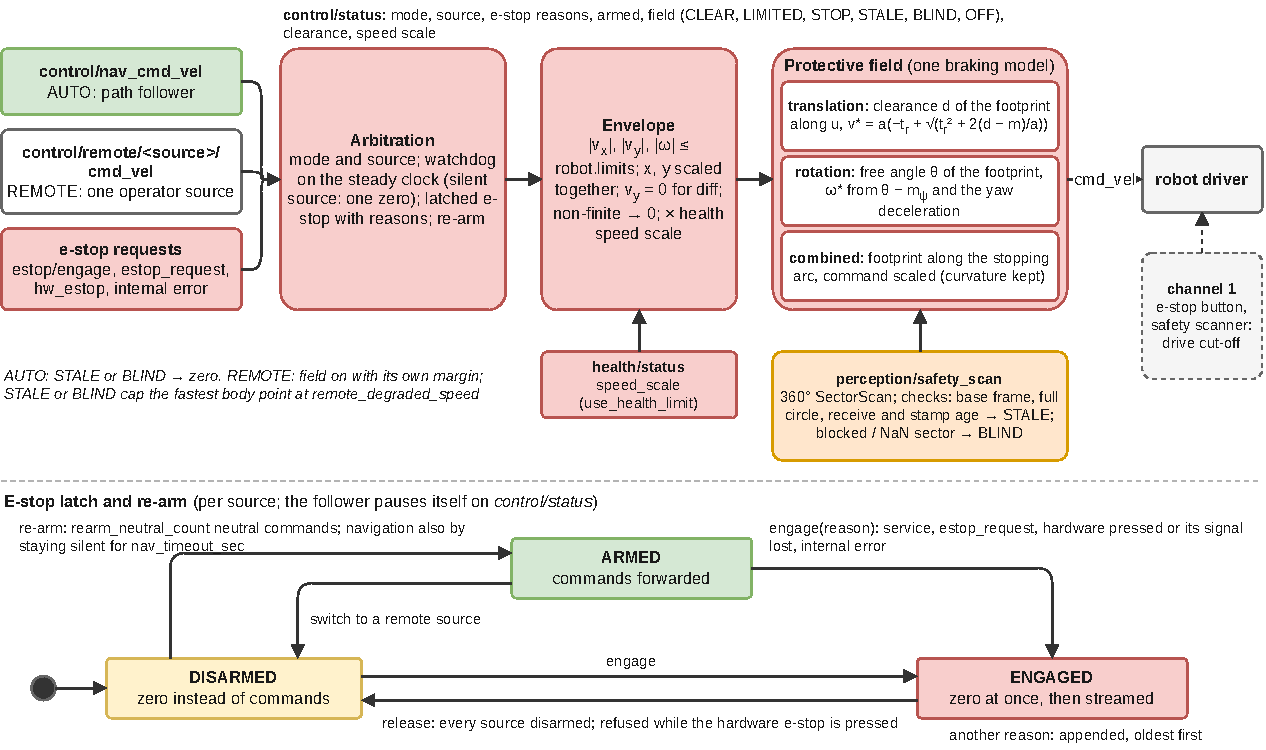
\includegraphics[width=0.9\textwidth]{safety_pipeline}
  \caption{Safety layer: arbitration, envelope and protective field in front of the robot's
    \topic{cmd\_vel}, and the e-stop latch with re-arm. Channel 1 (hardware) cuts the drive
    independently of any software.}
  \label{fig:safety}
\end{figure*}

The control multiplexer (Fig.~\ref{fig:safety}) arbitrates navigation (AUTO) and one operator
source (REMOTE) with watchdogs on the steady clock, clamps every command to the robot's
envelope (non-finite values become zero) and limits it with a protective field on the 360°
safety scan, a form of speed and separation monitoring~\cite{isots15066,marvel2016ssm}.

\textbf{Translation.} For the direction $\hat{\vect{u}}$ of the commanded translation, the
clearance $d_t$ is the distance the footprint can move before touching a scan point (points
ahead of the leading edge within the body corridor widened by a lateral margin, and zero for a
point beside or inside the body). The speed is scaled to $v^*(d_t - m)$, keeping the direction.

\textbf{Rotation.} Turning in place, the corners sweep the ring $r_{\mathrm{in}} < r \le
r_{\mathrm{c}}$ (0.28 to 0.49~m for the default profile), which the original field ignored. The
free angle $\theta_f$ is found by rotating the ring points in 1° steps until one enters the
footprint, and $|\omega| \le \omega^*(\theta_f - m_\psi)$ with the same model and the yaw
deceleration.

\textbf{Combined motion.} For a twist $(v_x, v_y, \omega)$ the robot keeps the command for
$\tr$ and then brakes both axes proportionally over $T_b = \max(v/a, |\omega|/\alpha)$; it
covers the constant-twist arc up to the parameter $u = \tr + T_b/2$ (exactly $D(v)$ on a
straight line). The footprint is checked at poses along the arc; if the first contact is at
$u_c$, scaling the command by $s$ keeps the curvature and covers $s\tr + s^2 T_b/2$, so the
largest clear scale is
\begin{equation}
  s = \frac{-\tr + \sqrt{\tr^2 + 2 T_b u_c}}{T_b}.
\end{equation}
With $a = 0.6$~m/s$^2$, $\tr = 0.25$~s and $m = 0.15$~m, \eqref{eq:braking} allows 0.30, 0.52,
0.87 and 1.35~m/s at 0.3, 0.5, 1.0 and 2.0~m of free distance.

\textbf{Fail-safe semantics.} A sector with no data is not free space. The perception node
reports every sector as \textsc{blocked} when the LiDAR is blind (too few points, or an empty
quarter of the view), when the sensor or levelling transform is missing, when processing fails
or when no usable cloud arrives; blocked and NaN sectors are obstacles at the robot for every
consumer. The mux accepts a scan only in the base frame with full-circle coverage and fresh
receive and stamp ages; otherwise it is \textsc{stale}. In AUTO a stale or blind scan stops the
robot; in REMOTE the fastest point of the body is capped at a creep speed. Perception levels
the points with roll and pitch of the base before the height band, since in \frm{base\_link} a
floor point at range $r$ enters the band when $r > (h + z_{\min})/\sin\vartheta$: 2.9~m at a
gait pitch of $\vartheta = 2^\circ$ with a 10~cm margin. A $k$-th nearest point per sector
($k = 2$) ignores single dust returns, and a short obstacle memory in \frm{odom} keeps objects
that drop below the lowest beam near the robot.

\textbf{E-stop.} The e-stop latches a list of reasons (service, topic, hardware input, lost
hardware signal, internal error); zero is published at once and streamed while engaged. Release
is refused while the hardware e-stop is pressed and disarms every source: a source drives again
only after a number of consecutive neutral commands, so a stick held during a release never
moves the robot. An exception in any callback engages the e-stop.

\subsection{Health and the TF latency budget}
\label{sec:health}

The follower stops when the robot pose is older than a limit. tf2 answers a lookup at the
latest common time of the chain, so with $E$ the dynamic edges and $\tau_e$ their stamps,
\begin{equation}
  \begin{aligned}
    \mathrm{age}(t) &= t_{\mathrm{now}} - \min_{e \in E} \tau_e\\
    &\approx \max_{e}\big(L^{\mathrm{acq}}_e + L^{\mathrm{proc}}_e + L^{\mathrm{tx}}_e +
    L^{\mathrm{q}}_e - \Delta_e\big) + \Delta_{\mathrm{c}} + T_{\mathrm{p}},
  \end{aligned}
  \label{eq:tfage}
\end{equation}
with acquisition, processing, transport and queueing latencies, the clock offsets $\Delta_e$
of the edge sources and $\Delta_{\mathrm{c}}$ of the consumer, and $T_{\mathrm{p}}$ the time
since the last sample. In Dharma the LIO edge dominates: a 100~ms scan, 20--80~ms of processing and transport
give a normal age of about 0.15--0.35~s against a 0.5~s limit, and an unsynchronized LiDAR
clock adds its offset directly. The follower therefore distinguishes \textsc{tf\_starting},
\textsc{tf\_stale} and \textsc{tf\_clock} (a pose from the future) and, for ages between
0.1~s and the limit, predicts the pose forward with the odometry twist instead of stopping.
The health monitor checks topic rates and header stamp ages (a 10~Hz topic with 2~s old stamps
is a fault), per-edge TF ages to separate a clock offset (constant age) from load (growing
age), and requests a reduced speed scale from the mux when sensing degrades.
\todo{confirm the health checks against the finished dharma\_health 0.2.0}

\section{Software Engineering}
\label{sec:eng}

\textbf{Pure cores, thin nodes.} Every package has the same layout: \texttt{core/} holds the
algorithms, state machines and configuration dataclasses in plain Python and numpy, without
ROS imports; \texttt{utils/} holds the conversions between messages and core types; the nodes
only declare parameters, topics, services and timers. The path follower, for example, is a pure
state machine \texttt{Follower.tick(inputs)} $\to$ \texttt{Decision} (command, status, stop
events) with an explicit table of allowed state transitions; the node feeds it once per control
tick and publishes the decision, so every path through it, including zero commands on stop,
e-stop, stale inputs, pause and shutdown, is unit-tested without ROS. The original follower
node had 1429 lines; the new node has 277.

\textbf{Shared building blocks.} \pkg{dharma\_utils} provides what packages used to copy:
angles, quaternions, SE(2) and SE(3) helpers, filters (EMA, slew limiter, CUSUM), the typed
configuration, the robot profile, the braking model and swept-footprint clearances, atomic
files with backups and path guards, grid distance fields and the correlative matcher, the plugin
registry, structured logging, and \texttt{DharmaNode} (typed parameters with live validation,
TF cache with per-edge ages, exception-guarded timers, shutdown hooks).

\textbf{Checks.} A style test in every package enforces the conventions: modules of at most 300
lines (tests 400), no ROS imports in \texttt{core/}, no shadowed node members. Lint and format
run through the same pre-commit hooks locally and in CI (ruff, clang-format, prettier,
shellcheck). The CI workflow, identical in every repository, builds and tests on ROS~2 Foxy
(Python~3.8, numpy~1.17), Humble (Python~3.10, numpy~1.21) and Jazzy (Python~3.12, numpy~1.26);
Dharma dependencies are imported from \texttt{deps.repos} and checked out at the same branch when it exists, so a
change that spans repositories is tested together before it is merged.

\textbf{Traceability.} Two reviews of the original stack produced findings with priorities
(P0 safety, P1 robustness, P2 maintainability). Each one maps to a change and a regression test;
the technical manual lists the full table.

\begin{table}[t]
  \centering
  \caption{Engineering metrics before (v0.1) and after (v0.2.0)}
  \label{tab:metrics}
  \begin{tabular}{@{}lrr@{}}
    \toprule
    Metric & v0.1 & v0.2.0 \\
    \midrule
    Largest node (lines) & 1429 & 277 \\
    Copies of the node main boilerplate & 15 & 1 \\
    Copies of the latched QoS definition & 11 & 1 \\
    Robot geometry declared in (files) & $\approx 6$ & 1 \\
    Test functions (without lint) & 158 & 595 \\
    Findings with a cited test & -- & 90 of 97 \\
    CI distributions & 2 & 2 \\
    \bottomrule
  \end{tabular}
\end{table}

\section{Evaluation}
\label{sec:eval}

% Generated by experiments/report.py from experiments/results; do not edit.
\newcommand{\EOneMeasuredA}{0.04}
\newcommand{\EOneModelA}{0.08}
\newcommand{\EOneClearA}{0.17}
\newcommand{\EOneMeasuredB}{0.15}
\newcommand{\EOneModelB}{0.23}
\newcommand{\EOneClearB}{0.20}
\newcommand{\EOneMeasuredC}{0.32}
\newcommand{\EOneModelC}{0.45}
\newcommand{\EOneClearC}{0.22}
\newcommand{\EOneMeasuredD}{0.56}
\newcommand{\EOneModelD}{0.73}
\newcommand{\EOneClearD}{0.23}
\newcommand{\EOneStdMax}{0.012}
\newcommand{\EOneClearMin}{0.173}
\newcommand{\EOneReactMin}{0.02}
\newcommand{\EOneReactMax}{0.15}
\newcommand{\EOneRatioMax}{0.79}
\newcommand{\EOneRatioMin}{0.41}
\newcommand{\EOneZeroMeasuredA}{0.06}
\newcommand{\EOneZeroModelA}{0.08}
\newcommand{\EOneZeroClearA}{0.16}
\newcommand{\EOneZeroMeasuredB}{0.20}
\newcommand{\EOneZeroModelB}{0.23}
\newcommand{\EOneZeroClearB}{0.16}
\newcommand{\EOneZeroMeasuredC}{0.40}
\newcommand{\EOneZeroModelC}{0.45}
\newcommand{\EOneZeroClearC}{0.16}
\newcommand{\EOneZeroMeasuredD}{0.68}
\newcommand{\EOneZeroModelD}{0.73}
\newcommand{\EOneZeroClearD}{0.16}
\newcommand{\EOneZeroStdMax}{0.025}
\newcommand{\EOneZeroClearMin}{0.162}
\newcommand{\EOneZeroReactMin}{0.02}
\newcommand{\EOneZeroReactMax}{0.18}
\newcommand{\EOneZeroRatioMax}{0.97}
\newcommand{\EOneZeroRatioMin}{0.51}
\newcommand{\EOneHumanSpeed}{0.5}
\newcommand{\EOneRuns}{160}
\newcommand{\EOneCollisions}{0}
\newcommand{\ETwoRuns}{240}
\newcommand{\ETwoBlindZeroMax}{0.13}
\newcommand{\ETwoBlindDistanceMax}{0.28}
\newcommand{\ETwoSilentZeroMax}{0.55}
\newcommand{\ETwoCreepMax}{0.15}
\newcommand{\EThreeHardReplaceInliersRejected}{62}
\newcommand{\EThreeHardReplaceInliersAccepted}{38}
\newcommand{\EThreeHardReplaceInliers}{3453}
\newcommand{\EThreeHardReplaceOutliersRejected}{94}
\newcommand{\EThreeHardReplaceOutliersAccepted}{6}
\newcommand{\EThreeHardReplaceOutliers}{172}
\newcommand{\EThreeHardReplaceWorstMax}{1.93}
\newcommand{\EThreeEkfTagsInliersRejected}{3}
\newcommand{\EThreeEkfTagsInliersAccepted}{97}
\newcommand{\EThreeEkfTagsInliers}{2763}
\newcommand{\EThreeEkfTagsOutliersRejected}{79}
\newcommand{\EThreeEkfTagsOutliersAccepted}{21}
\newcommand{\EThreeEkfTagsOutliers}{125}
\newcommand{\EThreeEkfTagsWorstMax}{0.31}
\newcommand{\EThreeEkfTagsScanInliersRejected}{4}
\newcommand{\EThreeEkfTagsScanInliersAccepted}{96}
\newcommand{\EThreeEkfTagsScanInliers}{2763}
\newcommand{\EThreeEkfTagsScanOutliersRejected}{78}
\newcommand{\EThreeEkfTagsScanOutliersAccepted}{22}
\newcommand{\EThreeEkfTagsScanOutliers}{125}
\newcommand{\EThreeEkfTagsScanWorstMax}{0.12}
\newcommand{\EThreeScanRejected}{0.0}
\newcommand{\EThreeDistance}{86}
\newcommand{\EThreeRuns}{20}
\newcommand{\EFourCollisions}{0}
\newcommand{\EFourRuns}{120}
\newcommand{\EFiveNoneDone}{20}
\newcommand{\EFiveNoneTime}{24.5}
\newcommand{\EFiveNoneBacked}{0.01}
\newcommand{\EFiveNoneBlocked}{0.0}
\newcommand{\EFiveFreeDone}{20}
\newcommand{\EFiveFreeTime}{41.2}
\newcommand{\EFiveFreeBacked}{1.00}
\newcommand{\EFiveFreeBlocked}{0.0}
\newcommand{\EFivePersonDone}{20}
\newcommand{\EFivePersonTime}{35.4}
\newcommand{\EFivePersonBacked}{0.49}
\newcommand{\EFivePersonBlocked}{0.0}
\newcommand{\EFivePersonBackedMin}{0.04}
\newcommand{\EFivePersonBackedMax}{0.99}
\newcommand{\EFivePersonClearMin}{0.38}
\newcommand{\EFivePersonHeld}{0}
\newcommand{\EFiveWallClearMin}{0.41}
\newcommand{\EFiveCollisions}{0}
\newcommand{\EFiveRuns}{60}
\newcommand{\EFiveSeeds}{20}


\textbf{Simulation protocol.} E1--E4 close the loop over the pure cores at the node rates:
the simulator core moves an omnidirectional body with the acceleration limits of the profile
and detects collisions; its LiDAR follows the Mid-360 (vertical field of view from $-7^\circ$ to
$52^\circ$ at the mount height, range limits, noise); odometry drifts as $\T{odom}{base}
\leftarrow \T{odom}{base} \exp(\vect{\xi})$ with $\vect{\xi} \sim \mathcal{N}(\vect{0},
\boldsymbol{\Sigma}\,\Delta s)$ plus a yaw bias and a scale error; stamps lag by 50~ms (LiDAR)
and commands by 20~ms. Perception's sector pipeline and watchdog run at 10~Hz, the follower
with the bringup's reactive policy (VFH) at 20~Hz, and every command passes the mux's arbiter
and gate, in 10~ms ticks whose task phases are drawn from the seed. All parameters are the
package defaults with the default profile ($a = 0.6$~m/s$^2$, $\tr = 0.25$~s, field margin
$m = 0.15$~m); localization is the true pose except in E3, and the health scale and the
planner's replanning are not in the loop. Each condition runs seeds 1--20; tables give mean
$\pm$ standard deviation over the 20 runs unless stated. The scripts, worlds and raw results
are in \texttt{experiments/} of the hub; one command reruns them and regenerates the tables.

\textbf{E1: stopping distance.} The robot cruises at $v$ in AUTO (a command stream at 20~Hz)
when a person (radius 0.25~m) appears on its axis $D(v) + m$ ahead of the front edge, the
nearest appearance from which \eqref{eq:braking} still promises a stop with the margin.
Table~\ref{tab:stop} gives the distance from the first safety scan that shows the person to
standstill and the smallest clearance over all runs. The robot always stopped within $D(v)$
(at most \EOneRatioMax\,$D(v)$) and never closer than \EOneClearMin~m, with no collision in
\EOneRuns{} runs; the body started braking \EOneReactMin--\EOneReactMax~s after the person
appeared, inside $\tr$. The field spends almost the whole room because it lowers the speed
along $v^*(d)$ instead of braking at once; the margin holds because the simulated body brakes
at exactly $a$, which a real robot must be shown to reach.

\begin{table}[t]
  \centering
  \caption{E1: braking model $D(v)$, measured stopping distance (mean $\pm$ std) and smallest
    clearance (all 20 runs)}
  \label{tab:stop}
  % Generated by experiments/report.py from experiments/results; do not edit.
\begin{tabular}{@{}rrrrr@{}}
  \toprule
  $v_h$ (m/s) & $v$ (m/s) & $D(v)$ (m) & measured (m) & clearance (m) \\
  \midrule
    0.5 & 0.2 & 0.08 & 0.039 $\pm$ 0.003 & 0.173 \\
    0.5 & 0.4 & 0.23 & 0.145 $\pm$ 0.006 & 0.196 \\
    0.5 & 0.6 & 0.45 & 0.317 $\pm$ 0.009 & 0.219 \\
    0.5 & 0.8 & 0.73 & 0.558 $\pm$ 0.012 & 0.234 \\
    0.0 & 0.2 & 0.08 & 0.057 $\pm$ 0.007 & 0.163 \\
    0.0 & 0.4 & 0.23 & 0.196 $\pm$ 0.012 & 0.162 \\
    0.0 & 0.6 & 0.45 & 0.399 $\pm$ 0.018 & 0.163 \\
    0.0 & 0.8 & 0.73 & 0.679 $\pm$ 0.025 & 0.162 \\
  \bottomrule
\end{tabular}

\end{table}

\textbf{E2: blind LiDAR.} The robot drives at 0.5~m/s when the LiDAR fails for 4~s: silent (no
cloud), empty (clouds without points) or sparse (50 points, below the blindness threshold of
100). Table~\ref{tab:blind} gives, in AUTO, the time $t_0$ from the failure to the first zero
command and the distance $d$ to standstill, and in REMOTE the speed of the fastest body point
during the failure, against v0.1, re-implemented as a baseline (a blind cloud gave an all-zero
scan, which the field skipped as free; no perception watchdog; field off in REMOTE). v0.2
stops an empty or sparse scan within one scan period and a silent sensor at the 0.5~s
watchdog, and caps REMOTE at the creep speed; v0.1 drove on at full speed whenever clouds kept
arriving and in REMOTE.

\begin{table}[t]
  \centering
  \caption{E2: blind LiDAR in AUTO (time to zero command, distance to standstill) and REMOTE
    (largest settled creep speed of the fastest body point), 20 runs each}
  \label{tab:blind}
  % Generated by experiments/report.py from experiments/results; do not edit.
\begin{tabular}{@{}llrrr@{}}
  \toprule
  LiDAR & stack & $t_0$ (s) & $d$ (m) & creep (m/s) \\
  \midrule
    silent & v0.2 & 0.44 $\pm$ 0.04 & 0.43 $\pm$ 0.02 & 0.15 \\
    silent & v0.1 & 0.49 $\pm$ 0.04 & 0.46 $\pm$ 0.02 & 0.50 \\
    empty & v0.2 & 0.08 $\pm$ 0.03 & 0.25 $\pm$ 0.02 & 0.15 \\
    empty & v0.1 & never & $\ge$2.0 & 0.50 \\
    sparse & v0.2 & 0.08 $\pm$ 0.03 & 0.25 $\pm$ 0.02 & 0.15 \\
    sparse & v0.1 & never & $\ge$2.0 & 0.50 \\
  \bottomrule
\end{tabular}

\end{table}

\textbf{E3: localization.} The follower drives three laps (\EThreeDistance~m) of the mall
route of the simulator with the odometry drift of its drift scenario (1~cm$/\sqrt{\mathrm{m}}$,
$0.3^\circ/\sqrt{\mathrm{m}}$, 1\,\% scale, $0.1^\circ$/m yaw bias); four tags hang at the
corridor ends. A forward camera detects them at 5~Hz up to 5~m with the noise the tag source
assumes, and 5\,\% of the detections are outliers (heading 5--25$^\circ$, position
0.1--0.4~m off, like the pose ambiguity of a small tag). The three estimators get the same
odometry, detections and scans; scan matching runs at 1~Hz on the site map the simulator draws.
Table~\ref{tab:loc} and Fig.~\ref{fig:loc} show the errors against the true pose. Hard
replacement rejected \EThreeHardReplaceInliersRejected\,\% of the good detections, because
its 0.5~m threshold compares the change of \frm{map}$\to$\frm{odom}, which grows with the
distance from the odometry origin, and still accepted \EThreeHardReplaceOutliersAccepted\,\% of the outliers; the
chi-square gate rejected \EThreeEkfTagsOutliersRejected\,\% of the outliers and
\EThreeEkfTagsInliersRejected\,\% of the good detections, and no scan match
(\EThreeScanRejected\,\% rejected).

\begin{table}[t]
  \centering
  \caption{E3: localization error under seeded drift: RMSE of position (ATE), largest position
    error and RMSE of heading per run}
  \label{tab:loc}
  % Generated by experiments/report.py from experiments/results; do not edit.
\begin{tabular}{@{}lrrr@{}}
  \toprule
  Method & ATE (m) & max (m) & yaw (°) \\
  \midrule
    Hard replace (v0.1) & 0.430 $\pm$ 0.244 & 1.15 $\pm$ 0.42 & 3.27 $\pm$ 1.63 \\
    EKF, tags & 0.074 $\pm$ 0.009 & 0.21 $\pm$ 0.03 & 0.86 $\pm$ 0.21 \\
    EKF, tags + scan match & 0.028 $\pm$ 0.002 & 0.08 $\pm$ 0.01 & 0.46 $\pm$ 0.08 \\
  \bottomrule
\end{tabular}

\end{table}

\begin{figure}[t]
  \centering
  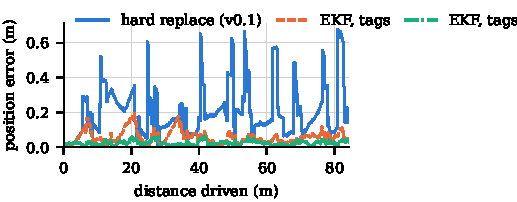
\includegraphics[width=\columnwidth]{figures/e3_error}
  \caption{E3, seed 1: position error over the distance driven.}
  \label{fig:loc}
\end{figure}

\textbf{E4: path shift.} The follower drives 20~m along the centre of a 3~m corridor: a person
stands on the route (\emph{on}) or both standing people stand 0.6--0.9~m beside it on opposite
sides (\emph{beside}), a third walks the same way at 0.2~m/s and a fourth crosses at 0.6~m/s
3~m ahead of the robot; people do not give way. Table~\ref{tab:shift} gives the completed runs,
their time, the stops before the goal, the smallest clearance to a person and the largest
distance from the route. \todo{E4 text}

\begin{table}[t]
  \centering
  \caption{E4: corridor with people (20 runs each): completed, time and stops (completed runs,
    mean $\pm$ std), smallest clearance and largest offset (all runs)}
  \label{tab:shift}
  \setlength{\tabcolsep}{3pt}
  % Generated by experiments/report.py from experiments/results; do not edit.
\begin{tabular}{@{}llrrrrr@{}}
  \toprule
  people & avoidance & done & time (s) & stops & clear. (m) & offset (m) \\
  \midrule
    on & path shift & 17/20 & 71.6 $\pm$ 1.7 & 1.2 $\pm$ 0.5 & 0.22 & 0.80 \\
    on & reactive & 0/20 & -- & -- & 0.35 & 0.01 \\
    on & none & 0/20 & -- & -- & 0.32 & 0.00 \\
    beside & path shift & 20/20 & 71.4 $\pm$ 1.7 & 1.2 $\pm$ 0.6 & contact & 0.79 \\
    beside & reactive & 13/20 & 70.9 $\pm$ 1.6 & 8.2 $\pm$ 2.4 & 0.12 & 0.00 \\
    beside & none & 13/20 & 70.9 $\pm$ 1.7 & 7.8 $\pm$ 1.9 & 0.12 & 0.00 \\
  \bottomrule
\end{tabular}

\end{table}

\textbf{End to end.} \todo{e2e}

\section{Limitations}
\label{sec:limits}

\textbf{Software safety is not certified.} The protective field, watchdogs and e-stop run in
Python over DDS. They are a second channel; a robot in a public space needs a first channel
that is safety-rated (hardware e-stop and a certified safety scanner or bumper wired to the
drive's safe torque off), designed and validated to ISO 13849-1~\cite{iso13849} or IEC
61508~\cite{iec61508}, and a safety case (hazards, mitigations, verification). Dharma reads the
hardware e-stop state so both channels latch together, but it does not replace it.

\textbf{Perception gaps.} A Mid-360 sees down to $-7^\circ$: mounted 0.53~m above the floor, a
10~cm object is seen only beyond about 3.5~m. The obstacle memory keeps objects seen before, but
an object that appears inside this near-field zone is not detected, and missing floor (stairs
down, platform edges) is not an obstacle at all. A pitched mount or a near-field sensor is
required where this matters. The scan is not deskewed (up to $v \cdot 0.1$~m of distortion per
frame), which the field margins must cover.

\textbf{No loop closure.} Mapping integrates scans at the corrected odometry pose; large sites
accumulate error between fiducials. A pose graph over scan matches with tags as landmarks would
unify mapping and localization.

\textbf{Sim-to-real gap.} The evaluation is in simulation with modelled drift, latency and
dropout. Braking deceleration and reaction time must be measured on each robot (worst-case
floor, payload and battery) before the field limits can be trusted; the results do not
transfer to another robot without repeating them, and real-robot trials are future work.

\section{Conclusion}
\label{sec:conclusion}

Dharma shows that a small autonomy stack can be both robot-agnostic and explicit about its
assumptions: one robot profile feeds every geometric and dynamic limit, the localization
estimate carries its uncertainty and gates its corrections, and a single braking model bounds
every speed from the route profile to the protective field, which treats missing data as an
obstacle. Pure algorithm cores and enforced conventions keep these models consistent across
eleven repositories and two ROS~2 distributions. \todo{summary of the measured results}
Future work is a pose graph for mapping and localization, deskewed and ground-segmented
perception for the near field, and a second robot model that runs the stack with only a new
robot adapter.


\bibliographystyle{IEEEtran}
\bibliography{references}

\end{document}
